\documentclass[12pt]{article}
\usepackage{amsmath,amssymb,amsthm}
\usepackage{graphicx,mathabx}
\usepackage{xcolor}
\usepackage{tikz}
\usepackage{placeins}
\usepackage{lipsum}
\usepackage[shortlabels]{enumitem}
\usepackage{wrapfig}
\begin{document}
\title{TCSS 343 - Week 1}
\author{Jake McKenzie}
\maketitle
\noindent\centerline{\textbf{Asymptotics with Divide and Conquer}}\\\\\\\\\\\\\\\\
\begin{center}
    ``You're always you, and that don't change, and you're always changing, and there's nothing you can do about it." \\$\dots$\\ Neil Gaiman
\end{center}
\begin{center}
    ``If one proves the equality of two numbers $a$ and $b$ by showing first that $a \leq b$ and then that $b \geq a$, it is unfair; one should instead show that they are really equal by disclosing the inner ground for their equality". \\$\dots$\\Emmy Noether
\end{center}
\begin{center}
    ``You shouldn't try optimizing something that you can't measure." \\$\dots$\\ Elecia White
\end{center}
\newpage
Exact answers are nice when you can find them. Often times we can't or don't care to find them. As computer scientists we care about the behaivor of the algorithms we employ. If we run into a recurrence relation or summation that expressed loosly the behaivor of these algorithms we'd like to know something about their runtime.\\\\
\centerline{\textbf{Asymptotic Notation in Seven Words}}\\
\centerline{\textbf{suppress constant factors and lower-order terms}}\\\\
Constant factors are things that will be language and system dependent while lower order terms are irrelevant for large inputs.\\\\
Now consider these definitions:\\
\textbf{Big-O Notation}\\
If $\lim\limits_{n\to\infty}{\frac{f(n)}{g(n)}}\to0$ then $f(n) \in O(g(n))$\\\\
This is another way of saying that $f(n) \leq c \cdot g(n)$ for some position $c$.\\
\textbf{Big-$\Omega$ Notation}\\
If $\lim\limits_{n\to\infty}{\frac{f(n)}{g(n)}}\to\infty$ then $f(n) \in \Omega(g(n))$\\\\
This is another way of saying that $f(n) \geq c \cdot g(n)$ for some position $c$.\\
\textbf{Big-$\Theta$ Notation}\\
If $\lim\limits_{n\to\infty}{\frac{f(n)}{g(n)}}\to k$ where k is a positive finite number then $f(n) \in \Theta(g(n))$\\\\
This is another way of saying that $f(n) \in O(g(n))$ and $f(n) \in \Omega(g(n))$\.\\
Now while we're in this course, we will typically need to show that these relationships are true when prompted, but it's always good to know that the following is true where \begin{math}0 < \epsilon < 1 < c\end{math}.\\
\[1 < \log{\log{n}} < \log{n} < n^{\epsilon} < n^c < n^{log{n}} < c^n < n^n < c^{c^{n}}\]\\
This asymptotic pecking order above is from Don Knuth's Concrete Mathematics.\\\\
\newpage
Now consider the following truths I found in Tim Roughgarden's Algorithms Illuminated: \\
$$\max\{f(n),g(n)\} \leq f(n) + g(n) \land  2 \cdot \max\{f(n),g(n)\} \geq f(n) + g(n)$$
(reminder that $\land$ is the logical ``and" symbol.)\\\\
1. Prove the following  by using the definitions that I've given prior and the information immediately above to show that $\max\{f(n),g(n)\}\in\Theta(f(n) + g(n))$
\newpage
\noindent 2. Arrange the following functions in order of increasing growth rate, with $g(n)$ following $f(n)$ 
in your list if and only if $f(n) \in O(g(n))$. That means using the limit definitions I gave you or by proof 
technique you've seen in class. You cannot simply use Don's asymptotic pecking order I stated but I strongly 
suggest you use the asymptotic pecking order as a guide to the neighborhood of a correct answer.\\
\begin{enumerate}[a)]
\item $\sum\limits_{i = 0}^{n} 2^i$\\
\item $n^2$\\
\item $n^{0.9999999}\log{n}$\\
\item $1.00001^n$\\
\item $4^{\log{n}}$\\
\item $100^{\sqrt{n}}$\\
\item $\log{2^{\frac{n}{2}}}$\\
\item $1000000n$\\
\end{enumerate}
\newpage
\noindent 3. Arrange the following functions in order of increasing growth rate, with $g(n)$ following $f(n)$ in your list if and only if $f(n) \in O(g(n))$. That means using the limit definitions I gave you or by proof technique you've seen in class. You cannot simply use Don's asymptotic pecking order I stated but I strongly suggest you use the asymptotic pecking order as a guide to the neighborhood of a correct answer.\\
\begin{enumerate}[a)]
\item  $n^{\frac{5}{3}}$\\
\item $\sum\limits_{i = 0}^{n} (i + 1)$\\
\item $n\sqrt{n}$\\
\item $\log{n^n}$\\
\item $(\frac{n}{\log{n}})^3$\\
\item  $2^{\frac{n}{2}}$\\
\item  $\log{\log{n}}$\\
\item  $n^{1.5}$\\
\end{enumerate}
\newpage
\noindent 4. Using what you know prove or disprove that  if $f(n) \in O(g(n)) $ and $g(n) \in O(f(n))$ then $f(n) = g(n) \forall n$.
\newpage
\noindent 5. Using what you know prove or disprove that $f(n) + O(f(n)) \in \Theta(f(n))$.
\newpage
\noindent 6. Using what you know prove or disprove that $f(n)\in O(f(n)^2)$.
\newpage
\noindent 7. Prove by induction that: $\sum\limits_{k=1}^{n}{\frac{k}{2^k}}=2-2^{1-n}-n2^{-n}$.
\newpage
\noindent 8. What is the code doing and from that information can you make a guess as to the worstcase runtime of this algorithm? (hint: follow what the code is doing by letting $x = 100$ and returning the result. You may use a calculator.)\\
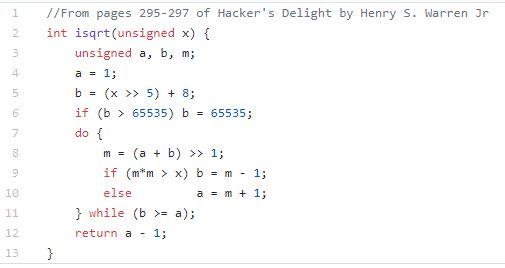
\includegraphics[width=\linewidth]{isqrt.jpg}
\newpage
\noindent So about that integer square root function on the previous page. If you said $O(\log{n})$ good job, you were really close. It actually has $O(\log{\log{n}})$ worst case runtime but degrades to $O(\log{n})$ given a bad initial guess. The choice of an initial guess is a deep and rich subject in it's own. There's a very famous algorithm, first discovered at Silicon Graphics in the 80's but popularized in the early aughts by a programmer on Usenet who worked at id Software, the creators of Quake. \\\\
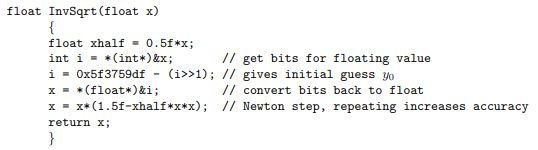
\includegraphics[scale =0.65]{fisqrt.jpg}  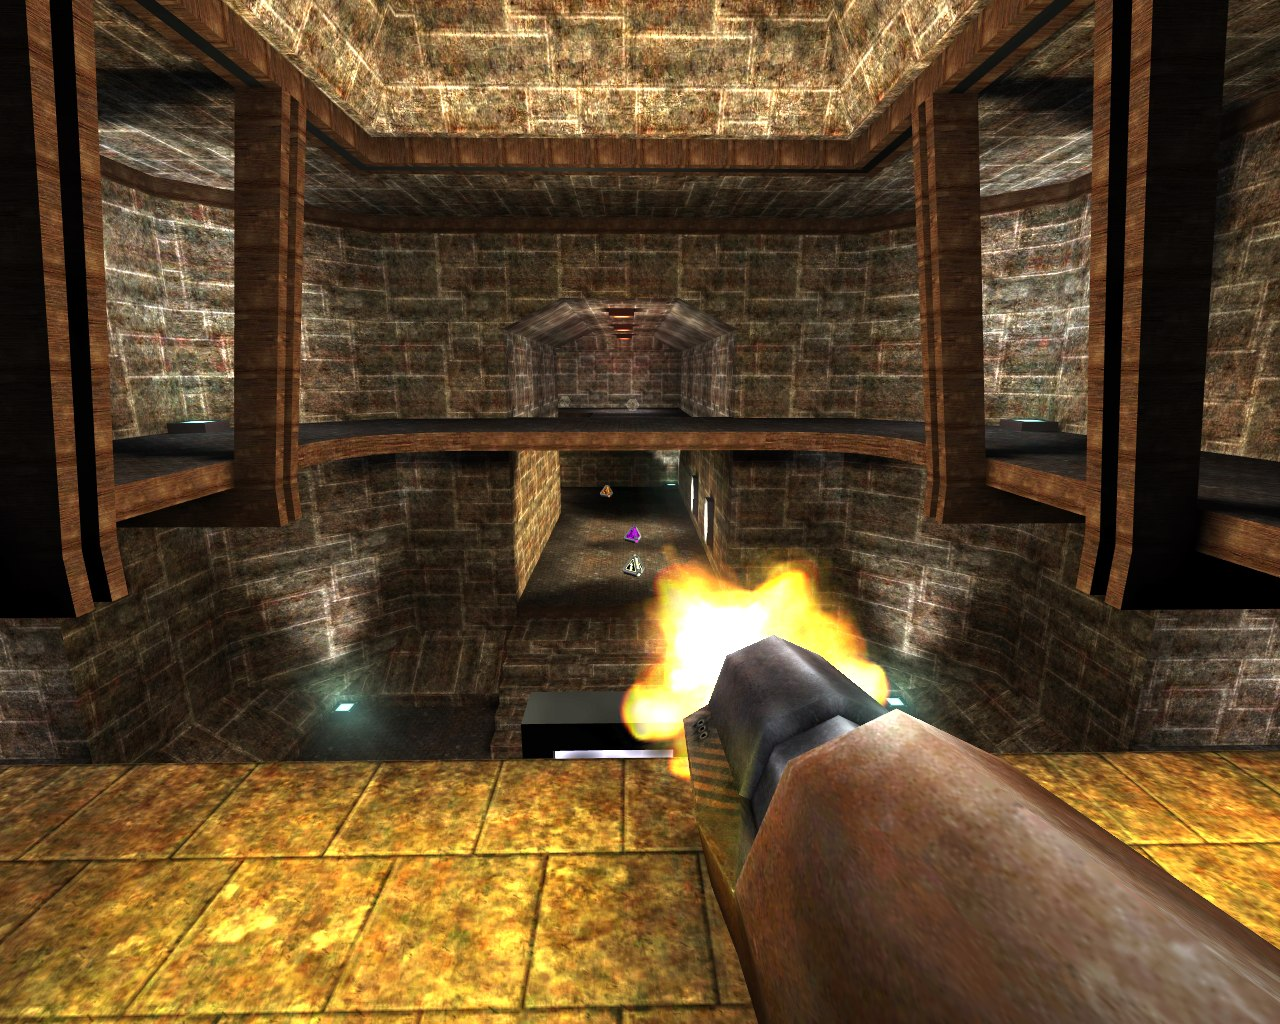
\includegraphics[scale =0.095]{qk.jpg}
\\\\Do you see that 0x$5$f$3759$df? That's known as the ``magic number" and offers a better than good initial guess for just about any number. The most absolute error fast inverse square root gives is $0.175\%$. This a deeply cherished algorithm and beloved number by anyone in computer graphics, but sadly hasn't gotten studied too much due to it being an insight found by industry professionals who desperately needed it.\\\\
I've actually been implementing my own square root algorithm in a HDL (hardware description language) and I encourage you to make your own personal projects. It need not be for anyone elses benefit or it very much may just be for others benefit!\\
\centerline{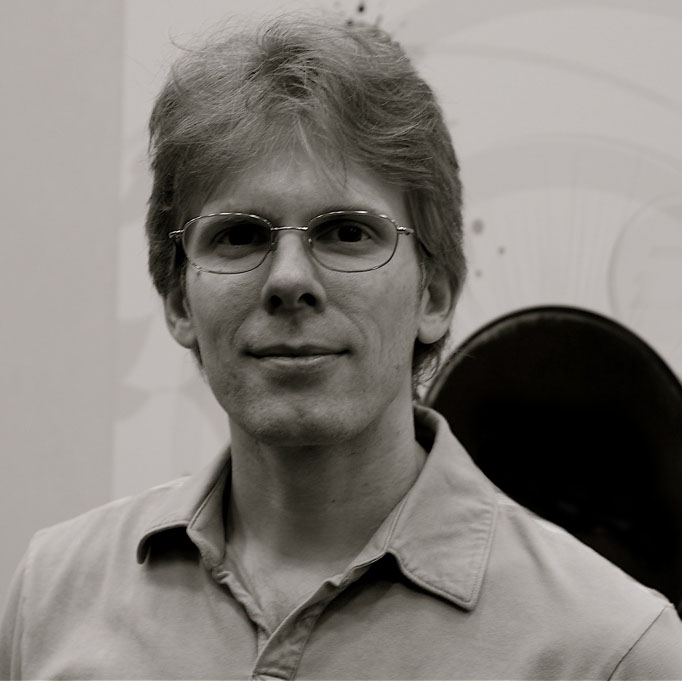
\includegraphics[scale =0.08]{jc.jpg}}\\
\centerline{John Carmack}
\\``In the information age, the barriers to entry into programming just aren't there. The barriers are self imposed. If you want to set off and go develop some grand new thing, you don't need millions of dollars of capitalization. You need enough pizza and Diet Coke to stick in your refrigerator, a cheap PC to work on, and the dedication to go through with it. We slept on floors. We waded across rivers."\\ 
\noindent If you were a bit confused and overwhelmed what I showed you in 8, please take a look at these. I wanted you to be able to look at some code and analyze it before presenting information as an oracle. Here is a simpler illustration to how the simple divide and conquer approach work. I think you should sit down and really try to understand why this example works as it does. It will help you going forward.\\\\
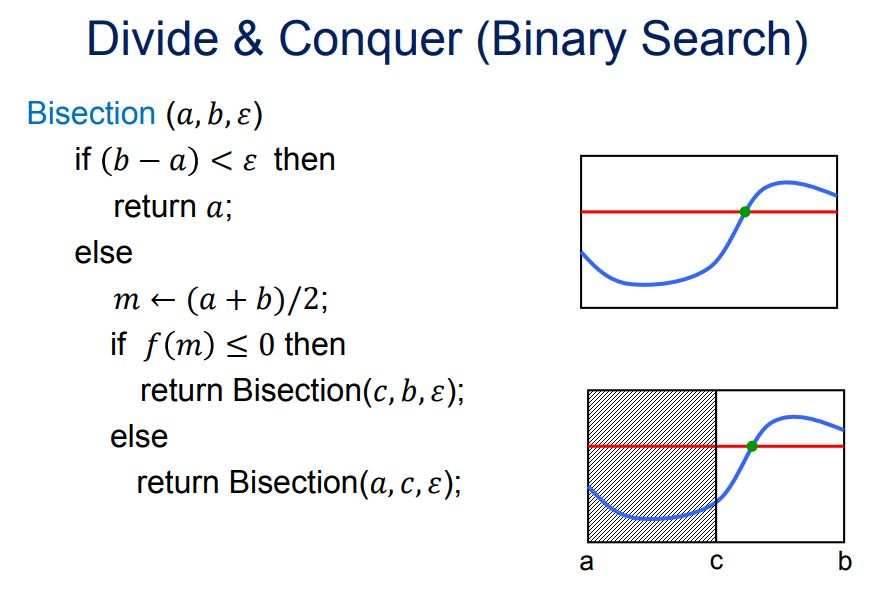
\includegraphics[scale =0.5]{bs.jpg}\\
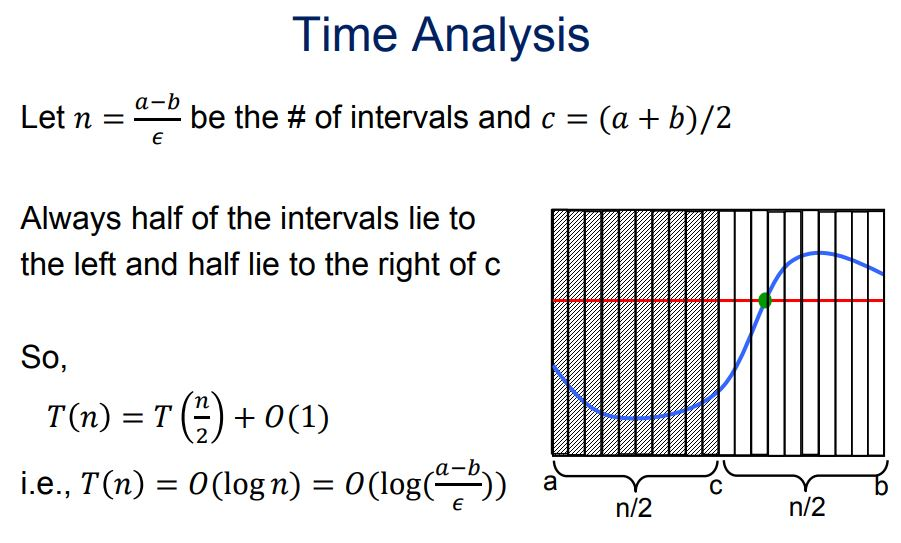
\includegraphics[scale =0.5]{bs2.jpg}\\
\newpage
\begin{wrapfigure}{R}{0.3\textwidth}
    \centering
    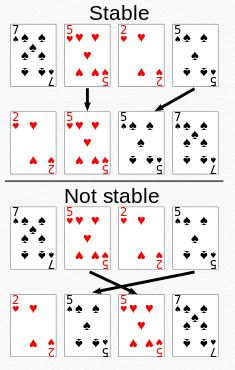
\includegraphics[width=0.325\textwidth]{ssort.jpg}
\end{wrapfigure}
\noindent A. Argue given what you know which of the following in the list of sorts given are stable or unstable. A sorting algorithm is said to be stable if two objects with equal keys appear in the same order in sorted output as they appear in the input array to be sorted.\\\\
\begin{enumerate}
    \item[a)]Randomized Quick Sort
    \item[b)]Bubble Sort
    \item[c)]Selection Sort
    \item[d)]Heap Sort
    \item[e)]Merge Sort
    \item[f)]Insertion Sort
\end{enumerate}
\noindent B. Using what you know prove or disprove that if $O(f(n)O(g(n)))\in O(f(n)g(n))$ then $O(f(n)g(n)) \in f(n)O(g(n))$.
\newpage
\noindent\textbf{Interview Question: Binary Search}\\
\noindent C. Given an already sorted ArrayList of integers write a function in Java that finds the value $t$ from $n$ keys via binary search. Return $-1$ if $t$ is not in the list otherwise return the index.\\
\newpage
\noindent D. This problem is concerned with computing all permutations of an array. For example,
if the array is $(2,3,5, 7)$ one output could be $(2,3,5, 7)$, $(2,3,7,5)$, $(2,5,3, 7)$, $(2,5, 7,3)$,
$(2,7,3,5)$, $(2,7,5,3)$, $(3,2,5,7)$, $(3,2,7,5)$, $(3,5,2,7)$, $(3,5,7,2)$, $(3,7,2,5)$, $(3,7,5,2)$,
$(5, 2,3, 7)$, $(5,2,7,3)$, $(5,3,2,7)$, $(5,3,7,2)$, $(5,7,2,3)$, $(5,7,2,3)$, $(7,2,3,5)$, $(7,2,5,3)$,
$(7,3, 2,5)$, $(7,3,5, 2)$, $(7,5, 2,3)$, $(7,5,3, 2)$. (Any other ordering is acceptable too.)\\\\
Write a program which takes as input an array of distinct integers and generates all
permutations of that array. No permutation of the array may appear more than once.
Hint: How many possible values are there for the first element? Runtime?\\
\end{document}